\chapter{Reports}

TACC includes many reports for retrieving both financial data as well as
customer care information.  This chapter will focus primarily on the
general reporting features as well as some of the reports specific to
accounting.

\section{General Reporting Features}

Most reports in TACC are available from the TACC main menu from the
{\emph Reports} menu.

All reports within TACC have a consistent layout with the following items:
\begin{itemize}
\item A Date bar.  If a report allows a specific date range, the date
bar will be available at the top of the report.
\item The Report Title.  This will usually contain the title of the
report and possibly the dates displayed or other report specific
information.
\item The Report Body.  This contains the actual report data, specific
to each report.  Most reports can be sorted by clicking on the column
header.  Double clicking an item in the report body will usually "drill
down" to the item detail or open the corresponding Customer's window.
This functionality varies from report to report.
\item Control Buttons.  The buttons vary from report to report, the
following buttons are usually available:
\begin{itemize}
\item {\bf Filters} - Brings up a list of filters to customize the
appearance or contents of the report.
\item {\bf Refresh} - Forces the report body to be repopulated.
\item {\bf Print} - Brings up a print dialog allowing the report to be
printed to a printer or file.
\item {\bf Email} - Brings up an email dialog that allows you to enter
the email address you wish the report to be sent to, optionally
including a plain-text formatted report and CSV file which is suitable
for importing into a spreadsheet program such as Excel or OpenOffice
Calc.
\item {\bf Close} - Closes the report.
\end{itemize}
Reports can also have additional control buttons specific to that
particular report.
\end{itemize}


\begin{figure}[hbtp]
\center{ \fbox{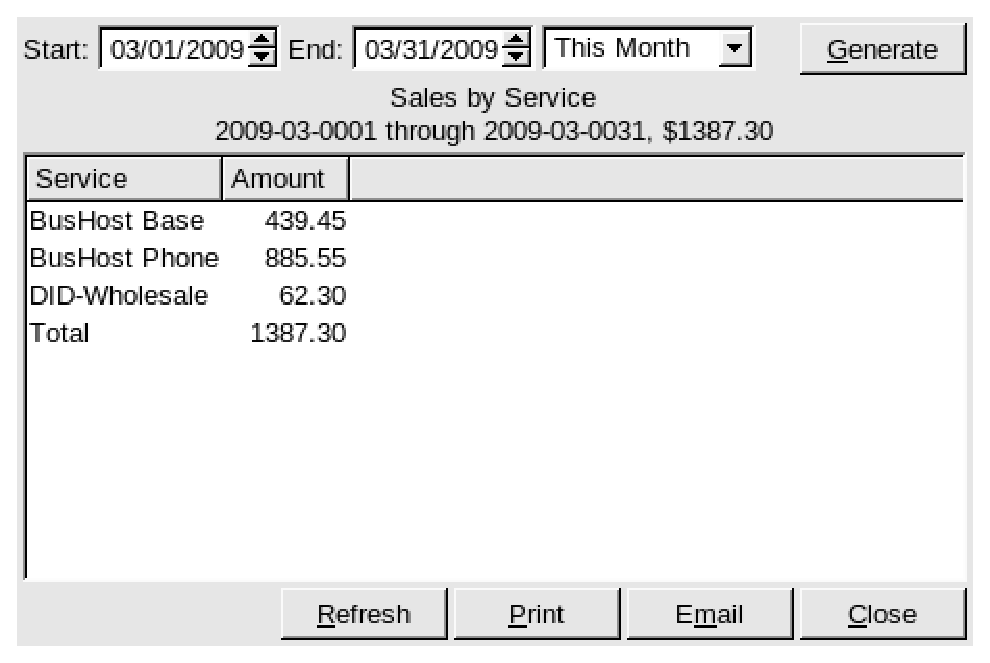
\includegraphics[width=7cm]{figures/SampleReport.eps}} }
\caption{ \label{fig:SampleReport} Sample Report }
\end{figure}



\section{General Ledger Report}

The General Ledger Report in TACC has the ability to display all items
that are posted into the General Ledger in both summary and detail form.

It is accessed from the {\emph Reports} menu by selecting {\emph General
Ledger}.  When first accessed, the report will display a summary of all
of the accounts in the Chart of Accounts and summarize the transaction
amounts for the current month.  See figure
~\ref{fig:GeneralLedgerReport} on page
~\pageref{fig:GeneralLedgerReport} for a sample General Ledger Report.

\begin{figure}[hbtp]
\center{ \fbox{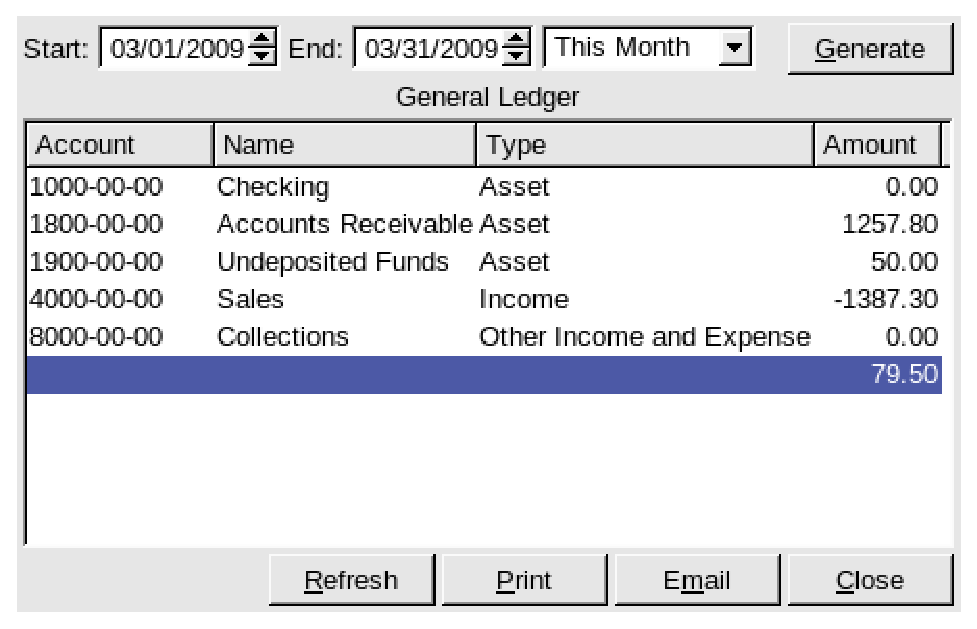
\includegraphics[width=7cm]{figures/GeneralLedgerReport.eps}} }
\caption{ \label{fig:GeneralLedgerReport} Sample General Ledger Reort}
\end{figure}

The General Ledger Report displays the following columns:
\begin{itemize}
\item {\bf Account} - This is the account number defined in the Chart of
Accounts (see ~\ref{Chart of Accounts} on page ~\pageref{Chart of Accounts}
for additional information).
\item {\bf Name} - The name of the account as defined in the Chart of
Accounts.
\item {\bf Type} - The type of account as defined in the Chart of
Accounts.
\item {\bf Amount} - What has posted to this account during the date
range specified in the report's Date Bar.
\end{itemize}

To view the individual transactions for a General Ledger account, double
click on the report item.  This will create a General Ledger detail
report for the selected account with the dates specified in the Date
Bar.

\section{General Ledger Detail Report}

